
%% bare_conf_compsoc.tex
%% V1.4b
%% 2015/08/26
%% by Michael Shell
%% See:
%% http://www.michaelshell.org/
%% for current contact information.
%%
%% This is a skeleton file demonstrating the use of IEEEtran.cls
%% (requires IEEEtran.cls version 1.8b or later) with an IEEE Computer
%% Society conference paper.
%%
%% Support sites:
%% http://www.michaelshell.org/tex/ieeetran/
%% http://www.ctan.org/pkg/ieeetran
%% and
%% http://www.ieee.org/

%%*************************************************************************
%% Legal Notice:
%% This code is offered as-is without any warranty either expressed or
%% implied; without even the implied warranty of MERCHANTABILITY or
%% FITNESS FOR A PARTICULAR PURPOSE! 
%% User assumes all risk.
%% In no event shall the IEEE or any contributor to this code be liable for
%% any damages or losses, including, but not limited to, incidental,
%% consequential, or any other damages, resulting from the use or misuse
%% of any information contained here.
%%
%% All comments are the opinions of their respective authors and are not
%% necessarily endorsed by the IEEE.
%%
%% This work is distributed under the LaTeX Project Public License (LPPL)
%% ( http://www.latex-project.org/ ) version 1.3, and may be freely used,
%% distributed and modified. A copy of the LPPL, version 1.3, is included
%% in the base LaTeX documentation of all distributions of LaTeX released
%% 2003/12/01 or later.
%% Retain all contribution notices and credits.
%% ** Modified files should be clearly indicated as such, including  **
%% ** renaming them and changing author support contact information. **
%%*************************************************************************


% *** Authors should verify (and, if needed, correct) their LaTeX system  ***
% *** with the testflow diagnostic prior to trusting their LaTeX platform ***
% *** with production work. The IEEE's font choices and paper sizes can   ***
% *** trigger bugs that do not appear when using other class files.       ***                          ***
% The testflow support page is at:
% http://www.michaelshell.org/tex/testflow/



\documentclass[conference,compsoc]{IEEEtran}
% Some/most Computer Society conferences require the compsoc mode option,
% but others may want the standard conference format.
%
% If IEEEtran.cls has not been installed into the LaTeX system files,
% manually specify the path to it like:
% \documentclass[conference,compsoc]{../sty/IEEEtran}





% Some very useful LaTeX packages include:
% (uncomment the ones you want to load)


% *** MISC UTILITY PACKAGES ***
%
%\usepackage{ifpdf}
% Heiko Oberdiek's ifpdf.sty is very useful if you need conditional
% compilation based on whether the output is pdf or dvi.
% usage:
% \ifpdf
%   % pdf code
% \else
%   % dvi code
% \fi
% The latest version of ifpdf.sty can be obtained from:
% http://www.ctan.org/pkg/ifpdf
% Also, note that IEEEtran.cls V1.7 and later provides a builtin
% \ifCLASSINFOpdf conditional that works the same way.
% When switching from latex to pdflatex and vice-versa, the compiler may
% have to be run twice to clear warning/error messages.



\usepackage{graphicx}


% *** CITATION PACKAGES ***
%
\ifCLASSOPTIONcompsoc
  % IEEE Computer Society needs nocompress option
  % requires cite.sty v4.0 or later (November 2003)
  \usepackage[nocompress]{cite}
\else
  % normal IEEE
  \usepackage{cite}
\fi
% cite.sty was written by Donald Arseneau
% V1.6 and later of IEEEtran pre-defines the format of the cite.sty package
% \cite{} output to follow that of the IEEE. Loading the cite package will
% result in citation numbers being automatically sorted and properly
% "compressed/ranged". e.g., [1], [9], [2], [7], [5], [6] without using
% cite.sty will become [1], [2], [5]--[7], [9] using cite.sty. cite.sty's
% \cite will automatically add leading space, if needed. Use cite.sty's
% noadjust option (cite.sty V3.8 and later) if you want to turn this off
% such as if a citation ever needs to be enclosed in parenthesis.
% cite.sty is already installed on most LaTeX systems. Be sure and use
% version 5.0 (2009-03-20) and later if using hyperref.sty.
% The latest version can be obtained at:
% http://www.ctan.org/pkg/cite
% The documentation is contained in the cite.sty file itself.
%
% Note that some packages require special options to format as the Computer
% Society requires. In particular, Computer Society  papers do not use
% compressed citation ranges as is done in typical IEEE papers
% (e.g., [1]-[4]). Instead, they list every citation separately in order
% (e.g., [1], [2], [3], [4]). To get the latter we need to load the cite
% package with the nocompress option which is supported by cite.sty v4.0
% and later.





% *** GRAPHICS RELATED PACKAGES ***
%
\ifCLASSINFOpdf
  % \usepackage[pdftex]{graphicx}
  % declare the path(s) where your graphic files are
  % \graphicspath{{../pdf/}{../jpeg/}}
  % and their extensions so you won't have to specify these with
  % every instance of \includegraphics
  % \DeclareGraphicsExtensions{.pdf,.jpeg,.png}
\else
  % or other class option (dvipsone, dvipdf, if not using dvips). graphicx
  % will default to the driver specified in the system graphics.cfg if no
  % driver is specified.
  % \usepackage[dvips]{graphicx}
  % declare the path(s) where your graphic files are
  % \graphicspath{{../eps/}}
  % and their extensions so you won't have to specify these with
  % every instance of \includegraphics
  % \DeclareGraphicsExtensions{.eps}
\fi
% graphicx was written by David Carlisle and Sebastian Rahtz. It is
% required if you want graphics, photos, etc. graphicx.sty is already
% installed on most LaTeX systems. The latest version and documentation
% can be obtained at: 
% http://www.ctan.org/pkg/graphicx
% Another good source of documentation is "Using Imported Graphics in
% LaTeX2e" by Keith Reckdahl which can be found at:
% http://www.ctan.org/pkg/epslatex
%
% latex, and pdflatex in dvi mode, support graphics in encapsulated
% postscript (.eps) format. pdflatex in pdf mode supports graphics
% in .pdf, .jpeg, .png and .mps (metapost) formats. Users should ensure
% that all non-photo figures use a vector format (.eps, .pdf, .mps) and
% not a bitmapped formats (.jpeg, .png). The IEEE frowns on bitmapped formats
% which can result in "jaggedy"/blurry rendering of lines and letters as
% well as large increases in file sizes.
%
% You can find documentation about the pdfTeX application at:
% http://www.tug.org/applications/pdftex





% *** MATH PACKAGES ***
%
%\usepackage{amsmath}
% A popular package from the American Mathematical Society that provides
% many useful and powerful commands for dealing with mathematics.
%
% Note that the amsmath package sets \interdisplaylinepenalty to 10000
% thus preventing page breaks from occurring within multiline equations. Use:
%\interdisplaylinepenalty=2500
% after loading amsmath to restore such page breaks as IEEEtran.cls normally
% does. amsmath.sty is already installed on most LaTeX systems. The latest
% version and documentation can be obtained at:
% http://www.ctan.org/pkg/amsmath





% *** SPECIALIZED LIST PACKAGES ***
%
%\usepackage{algorithmic}
% algorithmic.sty was written by Peter Williams and Rogerio Brito.
% This package provides an algorithmic environment fo describing algorithms.
% You can use the algorithmic environment in-text or within a figure
% environment to provide for a floating algorithm. Do NOT use the algorithm
% floating environment provided by algorithm.sty (by the same authors) or
% algorithm2e.sty (by Christophe Fiorio) as the IEEE does not use dedicated
% algorithm float types and packages that provide these will not provide
% correct IEEE style captions. The latest version and documentation of
% algorithmic.sty can be obtained at:
% http://www.ctan.org/pkg/algorithms
% Also of interest may be the (relatively newer and more customizable)
% algorithmicx.sty package by Szasz Janos:
% http://www.ctan.org/pkg/algorithmicx




% *** ALIGNMENT PACKAGES ***
%
%\usepackage{array}
% Frank Mittelbach's and David Carlisle's array.sty patches and improves
% the standard LaTeX2e array and tabular environments to provide better
% appearance and additional user controls. As the default LaTeX2e table
% generation code is lacking to the point of almost being broken with
% respect to the quality of the end results, all users are strongly
% advised to use an enhanced (at the very least that provided by array.sty)
% set of table tools. array.sty is already installed on most systems. The
% latest version and documentation can be obtained at:
% http://www.ctan.org/pkg/array


% IEEEtran contains the IEEEeqnarray family of commands that can be used to
% generate multiline equations as well as matrices, tables, etc., of high
% quality.




% *** SUBFIGURE PACKAGES ***
%\ifCLASSOPTIONcompsoc
%  \usepackage[caption=false,font=footnotesize,labelfont=sf,textfont=sf]{subfig}
%\else
%  \usepackage[caption=false,font=footnotesize]{subfig}
%\fi
% subfig.sty, written by Steven Douglas Cochran, is the modern replacement
% for subfigure.sty, the latter of which is no longer maintained and is
% incompatible with some LaTeX packages including fixltx2e. However,
% subfig.sty requires and automatically loads Axel Sommerfeldt's caption.sty
% which will override IEEEtran.cls' handling of captions and this will result
% in non-IEEE style figure/table captions. To prevent this problem, be sure
% and invoke subfig.sty's "caption=false" package option (available since
% subfig.sty version 1.3, 2005/06/28) as this is will preserve IEEEtran.cls
% handling of captions.
% Note that the Computer Society format requires a sans serif font rather
% than the serif font used in traditional IEEE formatting and thus the need
% to invoke different subfig.sty package options depending on whether
% compsoc mode has been enabled.
%
% The latest version and documentation of subfig.sty can be obtained at:
% http://www.ctan.org/pkg/subfig




% *** FLOAT PACKAGES ***
%
%\usepackage{fixltx2e}
% fixltx2e, the successor to the earlier fix2col.sty, was written by
% Frank Mittelbach and David Carlisle. This package corrects a few problems
% in the LaTeX2e kernel, the most notable of which is that in current
% LaTeX2e releases, the ordering of single and double column floats is not
% guaranteed to be preserved. Thus, an unpatched LaTeX2e can allow a
% single column figure to be placed prior to an earlier double column
% figure.
% Be aware that LaTeX2e kernels dated 2015 and later have fixltx2e.sty's
% corrections already built into the system in which case a warning will
% be issued if an attempt is made to load fixltx2e.sty as it is no longer
% needed.
% The latest version and documentation can be found at:
% http://www.ctan.org/pkg/fixltx2e


%\usepackage{stfloats}
% stfloats.sty was written by Sigitas Tolusis. This package gives LaTeX2e
% the ability to do double column floats at the bottom of the page as well
% as the top. (e.g., "\begin{figure*}[!b]" is not normally possible in
% LaTeX2e). It also provides a command:
%\fnbelowfloat
% to enable the placement of footnotes below bottom floats (the standard
% LaTeX2e kernel puts them above bottom floats). This is an invasive package
% which rewrites many portions of the LaTeX2e float routines. It may not work
% with other packages that modify the LaTeX2e float routines. The latest
% version and documentation can be obtained at:
% http://www.ctan.org/pkg/stfloats
% Do not use the stfloats baselinefloat ability as the IEEE does not allow
% \baselineskip to stretch. Authors submitting work to the IEEE should note
% that the IEEE rarely uses double column equations and that authors should try
% to avoid such use. Do not be tempted to use the cuted.sty or midfloat.sty
% packages (also by Sigitas Tolusis) as the IEEE does not format its papers in
% such ways.
% Do not attempt to use stfloats with fixltx2e as they are incompatible.
% Instead, use Morten Hogholm'a dblfloatfix which combines the features
% of both fixltx2e and stfloats:
%
% \usepackage{dblfloatfix}
% The latest version can be found at:
% http://www.ctan.org/pkg/dblfloatfix




% *** PDF, URL AND HYPERLINK PACKAGES ***
%
%\usepackage{url}
% url.sty was written by Donald Arseneau. It provides better support for
% handling and breaking URLs. url.sty is already installed on most LaTeX
% systems. The latest version and documentation can be obtained at:
% http://www.ctan.org/pkg/url
% Basically, \url{my_url_here}.




% *** Do not adjust lengths that control margins, column widths, etc. ***
% *** Do not use packages that alter fonts (such as pslatex).         ***
% There should be no need to do such things with IEEEtran.cls V1.6 and later.
% (Unless specifically asked to do so by the journal or conference you plan
% to submit to, of course. )


% correct bad hyphenation here
\hyphenation{op-tical net-works semi-conduc-tor}


\begin{document}
%
% paper title
% Titles are generally capitalized except for words such as a, an, and, as,
% at, but, by, for, in, nor, of, on, or, the, to and up, which are usually
% not capitalized unless they are the first or last word of the title.
% Linebreaks \\ can be used within to get better formatting as desired.
% Do not put math or special symbols in the title.
\title{Bare Demo of IEEEtran.cls for\\ IEEE Computer Society Conferences}


% author names and affiliations
% use a multiple column layout for up to three different
% affiliations
\author{\IEEEauthorblockN{Isaac Sacramento\\ and Mauro Roisenberg\\ and Rodrigo Exterkoetter}
\IEEEauthorblockA{Departament of Computer Science\\
Federal University of Santa Catarina\\
Florianopolis, Santa Catarina\\
Email: isaac.sacramento@posgrad.ufsc.br}
\and
\IEEEauthorblockN{Leando P. de Figueiredo}
\IEEEauthorblockA{Departament of Physics\\
Federal University of Santa Catarina\\
Florianopolis, Santa Catarina\\
Email: homer@thesimpsons.com}}

% conference papers do not typically use \thanks and this command
% is locked out in conference mode. If really needed, such as for
% the acknowledgment of grants, issue a \IEEEoverridecommandlockouts
% after \documentclass

% for over three affiliations, or if they all won't fit within the width
% of the page (and note that there is less available width in this regard for
% compsoc conferences compared to traditional conferences), use this
% alternative format:
% 
%\author{\IEEEauthorblockN{Michael Shell\IEEEauthorrefmark{1},
%Homer Simpson\IEEEauthorrefmark{2},
%James Kirk\IEEEauthorrefmark{3}, 
%Montgomery Scott\IEEEauthorrefmark{3} and
%Eldon Tyrell\IEEEauthorrefmark{4}}
%\IEEEauthorblockA{\IEEEauthorrefmark{1}School of Electrical and Computer Engineering\\
%Georgia Institute of Technology,
%Atlanta, Georgia 30332--0250\\ Email: see http://www.michaelshell.org/contact.html}
%\IEEEauthorblockA{\IEEEauthorrefmark{2}Twentieth Century Fox, Springfield, USA\\
%Email: homer@thesimpsons.com}
%\IEEEauthorblockA{\IEEEauthorrefmark{3}Starfleet Academy, San Francisco, California 96678-2391\\
%Telephone: (800) 555--1212, Fax: (888) 555--1212}
%\IEEEauthorblockA{\IEEEauthorrefmark{4}Tyrell Inc., 123 Replicant Street, Los Angeles, California 90210--4321}}




% use for special paper notices
%\IEEEspecialpapernotice{(Invited Paper)}




% make the title area
\maketitle

% As a general rule, do not put math, special symbols or citations
% in the abstract
\begin{abstract}
In this paper we will present a new convolution neural network
model to deblurr post-insversion acoustic impedance images.

\end{abstract}

% no keywords




% For peer review papers, you can put extra information on the cover
% page as needed:
% \ifCLASSOPTIONpeerreview
% \begin{center} \bfseries EDICS Category: 3-BBND \end{center}
% \fi
%
% For peerreview papers, this IEEEtran command inserts a page break and
% creates the second title. It will be ignored for other modes.
\IEEEpeerreviewmaketitle



\section{Introduction}
%O problema
Deblurring is an important problem in image processing.
It seeks to remove distortions from a blurry image in order to
recover the original image. Recovering the original image
is possible if the details of the blurring method are known.
In most cases, blurred images lack of enough information
to uniquely recover a plausible image, this feature sets
deblurring as an ill-posed problem and characterizes as an inversion problem.
It is not observed in the literature a general object deblurring algorithm. Thus, as mentioned by \cite{Chrysos} exploiting domain-specific
knowledge can result in superior deblurring. The focus of this work is post-inversion acoustic impedance
deblurring. Specifically, acoustic impedance deblurring must take into account the fact that
the resulting image still must to reflect the synthetic seismic data characteristics.

Reservoir characterization consists in determining the multidimensional
and quantitative structure and properties of an oil field.
To achieve this goal, it is essential to combine in a single model
all the information, knowledge and data about the field, in such a
way that is possible to make the quantitative predictions about the reservoir behavior \cite{buiting}.
These data are usually geological models,
data logs, testimonial data, production summary and 3D seismic data. The seismic
amplitude is used in model generation and  reservoir characterization,
however, the deeper the investigated horizon is, the bigger the limit in using the seismic amplitude data \cite{riel}.
The seismic data inversion has proved to be an efficient tool to accurately integrate the seismic information
in order to generate models that contribute to an effective reservoir characterization \cite{sergio}.
Besides integrating data, seismic inversion is widely used because of its facility and precision
in interpreting the acoustic impedance.
According to \cite{Latimer}, a good acoustic impedance model contains more information
then the seismic data because this model keeps all the seismic data information and additional
information originated in the well-logs.
Depending on the applied method, the acoustic impedance volume is the result of
the integration of data from different sources, such as, the seismic data, well logs and
velocity models. Thus, building an acoustic impedance model is the natural process to 
integrate the available informations to obtain a model accessible to geophysicists, geologists
and engineers. 
The acoustic impedance models allow fast interpretations and an efficient identification of
exploratory targets in seismic scale. However, the seismic data are band-limited, in other words,
the seismic data are short of high and low frequencies. This is a consequence
of seismic acquisition, earth attenuation, high-frequency noise, etc \cite{xiaoiu}. This phenomenon leads
to a misinterpretation of seismic data and, by consequence, the same to the resulting acoustic
impedance models, that lacks of high-frequency details, additionally, inversion methods such as MAP (Maximum a posteriori),
lead to blurry images \cite{Levin}.
In this sense, we believe that increasing the resolution of the acoustic impedance models
through deblurring the model sections, as a post-inversion refining process, can lead to a more accurate
interpretation of the impedance models.

%A solução
We approach the problem of deblurring post-inversion acoustic impedance images through
the Convolution Neural Networks (CNN). CNN is a framework of deep learning which has been
used in a wide sort of machine learning tasks. The availability of benchmarks
\cite{Russakovsky} and the advances in Graphical Processing Unit (GPU) \cite{Buduma15}
allowed CNN to outperform techniques in detection \cite{Girshick,Bell}, model-free
tracking \cite{Nam}, classification \cite{He}. With excellence in feature learning,
CNN achieved notorious success in image classification \cite{Krizhevsky}, action
recognition \cite{S_Ji}, video classification \cite{AbdelHamid} and speech recognition \cite{Farfade}.
Under the post-inversion perspective, we consider acoustic impedance as image and work on it with
image processing algorithms.

In this paper we propose a new multilayer convolution network model to perform deblurring in post-inversion acoustic impedance.
Each network layer maps higher level features originated in the previews layers through convolutional filters.
To perform this mapping, the filters, also named weights, are adjusted by minimizing a loss function. The trained model enhances the
resolution of the impedance image, resulting in an equivalent image with increased high-frequency band and lower noise.
First, we blurr the synthetic acoustic impedance to form the pairs of images of high and low resolution. Then,
the dictionary of images is normalized to the real interval $[0,1]$ and used to train the convolutional model.
We compare the deblurred images depicted by our model and by two other deblurring methods ().
The core concept of our architecture is the combination of the convolution layers with regression
layers, thus proceeding a regression solution, instead of classification.
%\hfill mds
 
%\hfill August 26, 2015

\section{Related Work}
Deblurring plays an important role in computer vision.
Methods based on...However these methods lack
of ...

Recent researches in geophysics have applied deep learning solutions, such as convolution networks, to solve a wide
sort of problems such as lithofacies recognition \cite{qian} and calculation \cite{Liu}, 

However, there is a lack of researches to investigate methods for improving the resolution of
images resulting from inversion processes. Improving the resolution of seismic inversion is
possible by adding high frequency in acquisition and processing seismic data. The seismic data
is generally short of high and low frequencies and this phenomenon is caused by seismic acquisition,
earth attenuation, high-frequency noise, etc., what negatively influence on geologic interpretations of seismic data \cite{xiaoiu}.
Thus, we propose enhancing seismic impedance resolution adding high-frequency post-inversion through a convolutional
neural network.


\section{Data and Method}

\subsection{Acoustic Impedance Inversion}
The experiments described in this paper were performed
on a set of synthetic acoustic impedance images. Using synthetic models
is a common practice in reservoir characterization \cite{}. It allows to study the
results of the algorithms without external interferences and to obtain
efficient interpretations and assessments. 
According to \cite{Harvey}, wedge shaped models is a straight way to analysis the
seismic model modeling and inversion processes. It realistically reproduces
reservoir contexts such as stratigraphic refinements, \textit{pich-outs} in sand layers, 
edges and channel structures.

In order to generate a set of training images, we proceed two steps to obtain the wedge images.
In the fist step we create a set of random wedges forms, containing two horizontal dimensions represented in images 32 x 32.
The wedges representing the reservoir varied in width and length. The second step
filled the lithology with values of petrophysical properties. In order to simplify
the assessments and conclusions, the lithology structures are filled with constant
reference values of rock densities and compressional velocity observed in the literature.
With the density and velocity models the acoustic impedance is calculated and a high
resolution model is obtained. Fig. \ref{fig_lithology} illustrate the lithology
model with the corresponding values for density and velocity.
\begin{figure}[!t]
\centering
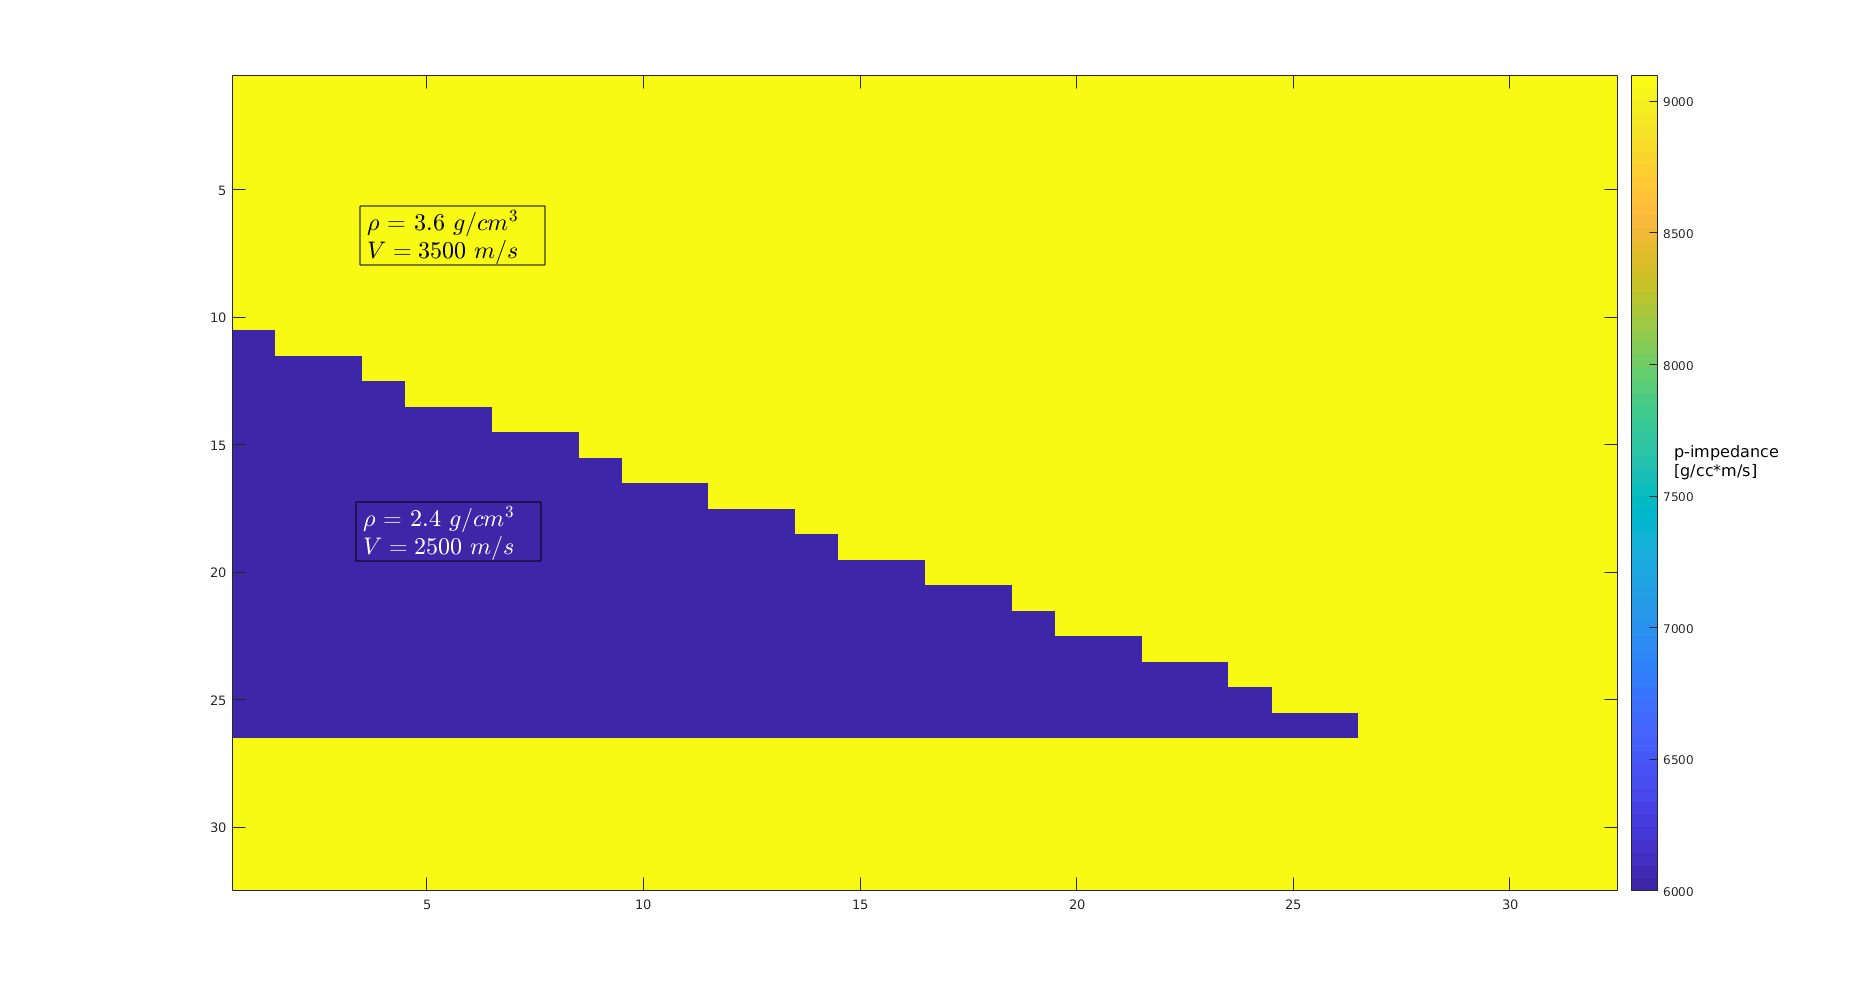
\includegraphics[width=3.0in]{Image_Paper}
\DeclareGraphicsExtensions.
\caption{Acoustic impedance blurred model.}
\label{fig_lithology}
\end{figure}

In a real scenario, the blurred acoustic impedance is the
result of an inversion method. However, for experimental purpose, the acoustic impedance models were low-passed filtered
and the high frequencies removed, this way we proceed the supervised training with high resolution and blurred images. The blurred image
is illustrated in Fig. \ref{Image_Paper_blurred}. To increase the number of examples in the training dataset we rotate the impedance models 
in angles countable multiples of 90 degrees. This approach allows the model to learn the maximum edges variability in wedges images.
\begin{figure}[!t]
\centering
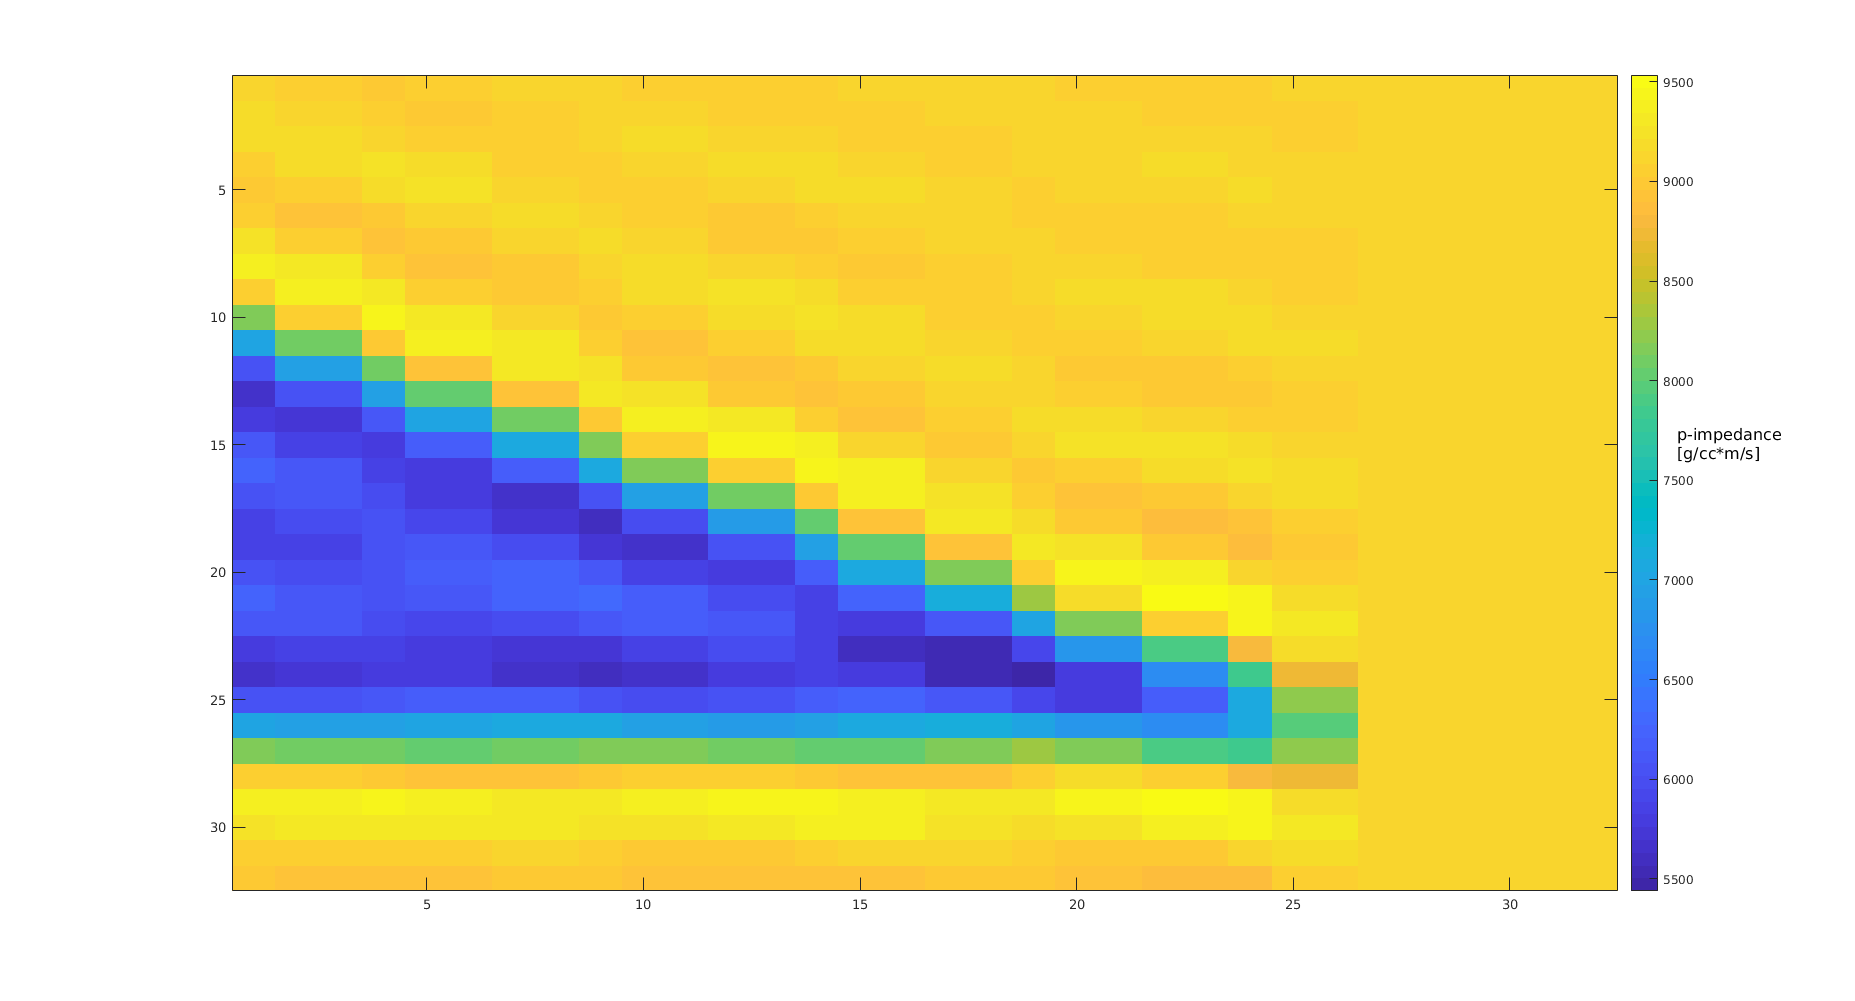
\includegraphics[width=3.0in]{Image_Paper_blurred}
\DeclareGraphicsExtensions.
\caption{Acoustic impedance blurred model.}
\label{fig_blur}
\end{figure}

\subsection{Convolutional Neural Network}
The work-flow of the proposed method consists of the following
steps:
\begin{itemize}
 \item Generate the synthetic impedance images;
 \item Blur these images through a low-pass filter;
 \item Train the convolutional model with the pair of high and low resolution images;
 \item Test the model with different blurry images;
 \item Assess the result for the testing output.
\end{itemize}

The approach adopted in this paper consists in training a CNN model to
to deblurr synthetic acoustic impedance images. The model
is able to solve two important problems related to deblurring physical properties
images: (1) learning the spacial patterns in the low resolution
training images and (2) predict each pixel intensity value in the new
higher resolution image. The CNN is a well established method for
patter recognition. Thus, an important breakthrough was developing a model
capable to proceed the regression task. To reach these two goals, the structure of the
model contains convolutional layers combined with a regression output
layer.

The model proceeds a supervised learning through the dictionary of pairs of low
and high resolution images. The optimization algorithm adjust the 
network weights in every layer by minimizing the Mean Squared Error (MSE)
in each batch of images. Thus, after the training phase, the model is capable
to deblurr any other image not presented in training dataset. The output
image recovers the high frequencies and presents higher similarity
to the high resolution image than to the blurred image according to a
specified metric. The model was adjusted to deblurr a wide variety
of wedges shapes and impedance values. Those wedges which the model was unable
to predict were added in the training set.

Three metrics assess the performance of the convolution networks: Fast Fourier Transform Index (FFTI),
the Rooted Mean Square Error (RMSE) and the frequencies magnitudes.
The FFTI is a similarity metric calculated based on the Fast Fourier Transform (FFT) of each image.
It is introduced by \cite{naranyana} and it is calculated as in Eq. \ref{eq:fourier}
\begin{equation}
 C = \frac{ (\sum_{i=1}^{N}{F_{1i}F_{2i}} - N \bar{F}_1\bar{F}_2 )^2 }{ (\sum_{i=1}^{N}{|F_{1i}|^2} - N{\bar{F}^2}_1)( \sum_{i=1}^{N}{|F_{2i}|^2} - N{\bar{F}^2}_2 )},
 \label{eq:fourier}
\end{equation}
where, for each frequency, an intensity value is calculated from the real and complex parts of fourier
transform. $F_{1i}$ represents the intensity value of $i$-th \textit{pixel} in the first image and $F_{2i}$
is the intensity value of $i$-th \textit{pixel} in the second image. $\bar{F}_1$ e $\bar{F}_2$ are the mean
frequencies in each image. The closer FFTI is to 1, the higher the similarity between the images.
The frequencies spectrum is additionally useful to present the graphic of frequency magnitudes in the images.
The frequency magnitude graphic allows distinguishing what high frequencies were added to the acoustic impedance
after the low resolution image is passed through the trained CNN. 
Additionally, the Root Mean Squared Error (RMSE) in Eq. \ref{eq:mse} is calculated in order to measure
the global error in each pair of deblurred and high resolution images.

\begin{equation}
 RMSE = \sqrt{\frac{ (\sum_{i=1}^{N}{(x_i -y_i)^2 } }{N}},
 \label{eq:mse}
\end{equation}

The model architecture consists in two convolution layers, each one followed by one
pooling layer and regularization layer. The second regularization layer is followed
by a fully connected layer, which maps the convolution layer's output to 1024 neurons.
The output model comprises a regression layer to predict the intensity value of each pixel.

\section{Experiments}
This section describes the implementation details and compares the proposed method  with the state-of-the-art
deblurring alritms in three different scenarios. The first scenario
evaluated the model capacity to deblurr lithologies with similar acoustic impedance
values as in the training dataset, but with different shapes.
This scenario allows assessing the generalization capacity of the model
to identify the lithology structure and deblurr the contours and edges.
The second scenario tested images with different acoustic impedance values and
different wedge shapes, in comparison to the ones the images used in the training phase.
In this case we tested the model capacity to deblurr the shapes of the wedges and
extrapolate the acoustic impedance values.

\subsection{Implementation Details}

% An example of a floating figure using the graphicx package.
% Note that \label must occur AFTER (or within) \caption.
% For figures, \caption should occur after the \includegraphics.
% Note that IEEEtran v1.7 and later has special internal code that
% is designed to preserve the operation of \label within \caption
% even when the captionsoff option is in effect. However, because
% of issues like this, it may be the safest practice to put all your
% \label just after \caption rather than within \caption{}.
%
% Reminder: the "draftcls" or "draftclsnofoot", not "draft", class
% option should be used if it is desired that the figures are to be
% displayed while in draft mode.
%
%\begin{figure}[!t]
%\centering
%\includegraphics[width=2.5in]{myfigure}
% where an .eps filename suffix will be assumed under latex, 
% and a .pdf suffix will be assumed for pdflatex; or what has been declared
% via \DeclareGraphicsExtensions.
%\caption{Simulation results for the network.}
%\label{fig_sim}
%\end{figure}

% Note that the IEEE typically puts floats only at the top, even when this
% results in a large percentage of a column being occupied by floats.


% An example of a double column floating figure using two subfigures.
% (The subfig.sty package must be loaded for this to work.)
% The subfigure \label commands are set within each subfloat command,
% and the \label for the overall figure must come after \caption.
% \hfil is used as a separator to get equal spacing.
% Watch out that the combined width of all the subfigures on a 
% line do not exceed the text width or a line break will occur.
%
%\begin{figure*}[!t]
%\centering
%\subfloat[Case I]{\includegraphics[width=2.5in]{box}%
%\label{fig_first_case}}
%\hfil
%\subfloat[Case II]{\includegraphics[width=2.5in]{box}%
%\label{fig_second_case}}
%\caption{Simulation results for the network.}
%\label{fig_sim}
%\end{figure*}
%
% Note that often IEEE papers with subfigures do not employ subfigure
% captions (using the optional argument to \subfloat[]), but instead will
% reference/describe all of them (a), (b), etc., within the main caption.
% Be aware that for subfig.sty to generate the (a), (b), etc., subfigure
% labels, the optional argument to \subfloat must be present. If a
% subcaption is not desired, just leave its contents blank,
% e.g., \subfloat[].


% An example of a floating table. Note that, for IEEE style tables, the
% \caption command should come BEFORE the table and, given that table
% captions serve much like titles, are usually capitalized except for words
% such as a, an, and, as, at, but, by, for, in, nor, of, on, or, the, to
% and up, which are usually not capitalized unless they are the first or
% last word of the caption. Table text will default to \footnotesize as
% the IEEE normally uses this smaller font for tables.
% The \label must come after \caption as always.
%
%\begin{table}[!t]
%% increase table row spacing, adjust to taste
%\renewcommand{\arraystretch}{1.3}
% if using array.sty, it might be a good idea to tweak the value of
% \extrarowheight as needed to properly center the text within the cells
%\caption{An Example of a Table}
%\label{table_example}
%\centering
%% Some packages, such as MDW tools, offer better commands for making tables
%% than the plain LaTeX2e tabular which is used here.
%\begin{tabular}{|c||c|}
%\hline
%One & Two\\
%\hline
%Three & Four\\
%\hline
%\end{tabular}
%\end{table}


% Note that the IEEE does not put floats in the very first column
% - or typically anywhere on the first page for that matter. Also,
% in-text middle ("here") positioning is typically not used, but it
% is allowed and encouraged for Computer Society conferences (but
% not Computer Society journals). Most IEEE journals/conferences use
% top floats exclusively. 
% Note that, LaTeX2e, unlike IEEE journals/conferences, places
% footnotes above bottom floats. This can be corrected via the
% \fnbelowfloat command of the stfloats package.




\section{Conclusion}
The conclusion goes here.




% conference papers do not normally have an appendix



% use section* for acknowledgment
\ifCLASSOPTIONcompsoc
  % The Computer Society usually uses the plural form
  \section*{Acknowledgments}
\else
  % regular IEEE prefers the singular form
  \section*{Acknowledgment}
\fi


The authors would like to thank...





% trigger a \newpage just before the given reference
% number - used to balance the columns on the last page
% adjust value as needed - may need to be readjusted if
% the document is modified later
%\IEEEtriggeratref{8}
% The "triggered" command can be changed if desired:
%\IEEEtriggercmd{\enlargethispage{-5in}}

% references section

% can use a bibliography generated by BibTeX as a .bbl file
% BibTeX documentation can be easily obtained at:
% http://mirror.ctan.org/biblio/bibtex/contrib/doc/
% The IEEEtran BibTeX style support page is at:
% http://www.michaelshell.org/tex/ieeetran/bibtex/
%\bibliographystyle{IEEEtran}
% argument is your BibTeX string definitions and bibliography database(s)
%\bibliography{IEEEabrv,../bib/paper}
%
% <OR> manually copy in the resultant .bbl file
% set second argument of \begin to the number of references
% (used to reserve space for the reference number labels box)
\begin{thebibliography}{1}

\bibitem{IEEEhowto:kopka} 	H.~Kopka and P.~W. Daly, \emph{A Guide to \LaTeX}, 3rd~ed.\hskip 1em plus 0.5em minus 0.4em\relax Harlow, England: Addison-Wesley, 1999.
\bibitem{xiaoiu}  		Xi Xiaoyu, Ling Yun, Sun Desheng, Guo Xiangyu, and Wang Huifeng, ``Studying the effect of expanding low or high frequency on post-stack seismic inversion,'' in SEG Technical Program Expanded Abstracts 2012. September 2012, 1-5.
\bibitem{Buduma15}  		Buduma, N., `` Fundamentals of Deep Learning,'' Academic Press, 2015, in O'Reilly Media.
\bibitem{qian} 			Qian Feng, Yin Miao, Su Ming-Jun, Wang Yaojun, Hu Guangmin, ``Seismic facies recognition based on prestack data using deep convolutional autoencoder,''.
\bibitem{Liu} 			Liu Lihui, Lu Rong, Li Jianhai, Yang Wenkui, ``Seismic Lithofacies Computation Method Based on Deep Learning,'' p. 649-652.
\bibitem{Chrysos} 		G. G. Chrysos, S. Zafeiriou, "Deep Face Deblurring," 2017 IEEE Conference on Computer Vision and Pattern Recognition Workshops (CVPRW), Honolulu, HI, 2017, pp. 2015-2024.
\bibitem{Latimer} 		Rebecca Buxton Latimer, Rick Davidson, Paul van Riel, ``An interpreter's guide to understanding and working with seismic-derived acoustic impedance data,'',2017, pp. 242-256, v. 19, num. 3, in The Leading Edge.
\bibitem{buiting} 		JJM. Buiting, M. Bacon,``Using geophysical, geological, and petrophysical data to characterize reservoirs in the North Sea.'', in 5th Conference on Petroleum Geology of NW Europe, London. CD-ROM.
\bibitem{riel} 			Paul van Riel,  ``The past, present and future of quantitative reservoir characterization.'', in The Leading Edge, 19, p. 878–881.
\bibitem{sergio}		Sergio Sacani Sancevero, Armando Zaupa Remacre, Rodrigo de Souza Portugal, ``O papel da inversão para a impedância no processo de caracterização sísmica de reservatórios'',in Revista Brasileira de Geofísica, 2006, p. 495-512, v. 24.
\bibitem{Russakovsky}		O. Russakovsky, J. Deng, H. Su, J. Krause, S. Satheesh, S. Ma, Z. Huang, A. Karpathy, A. Khosla, M. Bernstein, ``Imagenet large scale visual recognition challenge,'' in ternational Journal of Computer Vision (IJCV), p. 211–252, 2015.
\bibitem{Girshick}		R. Girshick, ``Fast r-cnn,'' In IEEE Proceedings of International Conference on Computer Vision (ICCV), pages 1440–1448, 2015.
\bibitem{Bell} 			S. Bell, C. L. Zitnick, K. Bala, and R. Girshick, ``Inside-outside net: Detecting objects in context with skip pooling and recurrent neural networks,'' in arXiv preprint arXiv:1512.04143, 2015.s
\bibitem{Nam}			H. Nam and B. Han, ``Learning multi-domain convolutional neural networks for visual tracking,'' In IEEE Proceedings of International Conference on Computer Vision and Pattern Recognition (CVPR). IEEE, 2016.
\bibitem{He}			K. He, X. Zhang, S. Ren, and J. Sun, ``Deep residual learning for image recognition,'' In IEEE Proceedings of International Conference on Computer Vision and Pattern Recognition (CVPR). IEEE, 2016.
\bibitem{Levin}			A. Levin, Y. Weiss, F. Durand, and W. T. Freeman. Understanding and evaluating blind deconvolution algorithms. In IEEE Proceedings of International Conference on Computer Vision and Pattern Recognition (CVPR), p. 1964–1971.
\bibitem{Krizhevsky}		A. Krizhevsky, I. Sutskever, G. E. Hinton, ``Imagenet classification with deep convolutional neural networks: Advances in neural information processing systems,'' 2012, p. 1097–1105.
\bibitem{S_Ji}			S. Ji,W. Xu, M. Yang, K. Yu, 2013, ``3d convolutional neural networks for human action recognition,'' in IEEE transactions on pattern analysis and machine intelligence, n. 35, p. 221–231.
\bibitem{AbdelHamid}		O. Abdel-Hamid, A.-r. Mohamed, H. Jiang, L. Deng, G. Penn, D. Yu, 2014, ``Convolutional neural networks for speech recognition,'' in IEEE/ACM Transactions on audio, speech, and language processing, n. 22, p. 1533–1545.
\bibitem{Farfade}		S. S. Farfade, M. J. Saberian, L.-J. Li, 2015, ``Multi-view face detection using deep convolutional neural networks,'' in Proceedings of the 5th ACM on International Conference on Multimedia Retrieval, ACM, p. 643–650.
\bibitem{Harvey} 		P. J. Harvey, D. J. MacDONALD, ``Seismic modelling of porosity within the jurassic aged carbonate bank, offshore Nova Scotia,'' in  Canadian Journal of Exploration Geophysics, n. 26, p. 54–71.
\bibitem{naranyana}		S. Narayana, P. K. Thirivikraman, ``Image similarity using fourier transform,'' in International Journal of Computer Engeneering and Technology, 2015, n. 6, p. 29–37.
\end{thebibliography}

%0 Journal Article
%A Rebecca Buxton Latimer
%A Rick Davidson
%A Paul van Riel
%T An interpreter's guide to understanding and working with seismic-derived acoustic impedance data
%D 2000
%J The Leading Edge
%P 242-256
%V 19
%N 3
%R 10.1190/1.1438580
%U http://library.seg.org/doi/abs/10.1190/1.1438580
%K 


% that's all folks
\end{document}


